\section{C1: where should the input enter?}\label{sec:c1}

\paragraph{Question and rule.} With the same frozen base maps, the same SFM context and a 140k-parameter conditioner, which entry point generalises best to unseen input shapes and sequences? Pre-registered rule (\node{C1-where}): a location is \emph{preferred} if it beats every other location with a paired 95\% CI excluding 0 on $\ge4/6$ dev plants, on \tier{shape\_ood} and \tier{sequence\_ood} separately, and is significantly worse on none. The weaker statement named by the hypothesis, ``weight-space (the better of HyperKKL and its dense ablation) beats both latent and concat on $\ge4/6$'', was pre-registered as the rule for the held-out plants (\node{TEST-C1}, run once with the frozen recipe).

\begin{figure}[t]
\centering
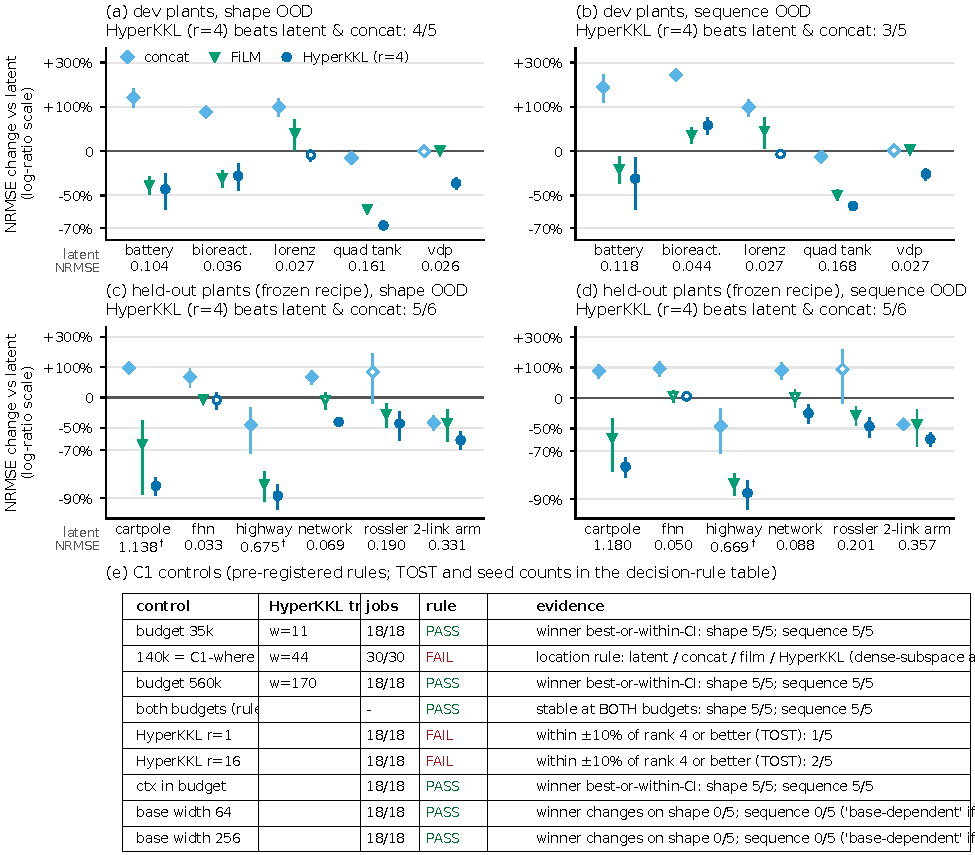
\includegraphics[width=0.68\textwidth, trim=0 171 0 0, clip]{fig1_c1_where.pdf}
\caption{C1, paired change in NRMSE relative to latent injection (the reference; its absolute NRMSE is printed under each plant). (a,b) dev plants, 5 seeds; (c,d) held-out plants, frozen recipe, 3 seeds. Filled markers: 95\% CI over seeds excludes 0; bars: 95\% CI. $\dagger$: latent injection itself above climatology. The pre-registered single-location rule fails on the dev plants (panel (e) of the generated figure, reproduced as Table~\ref{tab:decisions}); the weight-space-beats-latent-and-concat rule passes in all four panels.}
\label{fig:c1}
\end{figure}

\paragraph{Verdict: the pre-registered rule fails; the weaker claim holds and replicates.} No location is preferred (\node{C1-where}: \OutcomeCOneWhere; preferred location: \ConePreferredLocation): HyperKKL beats every other location on \ConeLoraBeatsAllShape\ plants (\tier{shape\_ood}) and \ConeLoraBeatsAllSeq\ (\tier{sequence\_ood}), its dense ablation on \ConeHyperBeatsAllShape\ and \ConeHyperBeatsAllSeq, and the two are within each other's CIs on most plants (Figure~\ref{fig:c1}; absolute NRMSE in Table~\ref{tab:c1}, Appendix~\ref{app:tables}). The weaker claim holds: weight-space beats both latent and concat on \ConeWeightSpaceBeatsLatConcShape\ (\tier{shape\_ood}) and \ConeWeightSpaceBeatsLatConcSeq\ (\tier{sequence\_ood}) plants. Read for HyperKKL alone ($r=4$) against latent injection: better on \ConeLoraBeatsLatentShape\ and worse on \ConeLoraLosesLatentShape\ plants on \tier{shape\_ood} (\ConeLoraVsLatentRangeShape\ where significant), better on \ConeLoraBeatsLatentSeq\ and worse on \ConeLoraLosesLatentSeq\ on \tier{sequence\_ood} (the loss is \sys{bioreactor}, where latent injection is best); FiLM is better on \ConeFilmBeatsLatentShape\ and worse on \ConeFilmLosesLatentShape, the additive residual \ConeConcatBeatsLatentShape\ and \ConeConcatLosesLatentShape. On the held-out plants (\node{TEST-C1}: \OutcomeTESTCOne) the weight-space claim holds on \CtestWeightSpaceBeatsLatConcShape\ and \CtestWeightSpaceBeatsLatConcSeq; HyperKKL alone beats latent injection on \CtestLoraBeatsLatentShape\ and \CtestLoraBeatsLatentSeq\ plants (\CtestLoraVsLatentRangeShape\ where significant), the exception being \sys{fhn}, where it is within CI of latent injection; latent injection is above climatology on \sys{cartpole} and \sys{highway\_traffic} (\tier{shape\_ood}), where HyperKKL is not. No single location passes the strict rule (\CtestPreferredLocation).
% TODO (results layer, single-method re-reading): replace the LoRA-named macros above by the
% 'hyperkkl' macros and add the HyperKKL-vs-concat count once generated; the weight-space verdicts
% (\ConeWeightSpaceBeatsLatConc*, \CtestWeightSpaceBeatsLatConc*) are the pre-registered ones.

\paragraph{Controls.} Each control is a pre-registered node whose counts are in Table~\ref{tab:decisions}. The ranking survives when the context encoder is charged to the budget (\node{C1-ctx}: \OutcomeCOneCtx) and across budgets of 35k and 560k (\node{C1-budget}: \OutcomeCOneBudget; an asterisk, where printed, marks a verdict decided while seeds were running). \emph{Rank ablation.} The rank is a real knob: $r=1$ and $r=16$ are not equivalent to $r=4$ at the $\pm10\%$ margin (\node{C1-rank1}: \OutcomeCOneRankOne, \node{C1-rank16}: \OutcomeCOneRankSixteen; Table~\ref{tab:decisions}), with $r=1$ losing accuracy on the chaotic and the oscillatory plant and $r=16$ non-inferior or better on half of them, consistent with $r$ trading regularisation against capacity; the default $r=4$ is the pre-registered setting, not a tuned one. Base-width controls (winner not base-dependent): \OutcomeCOneBasewidthSixtyFour\ / \OutcomeCOneBasewidthTwoFiveSix\ (jobs \JobsCOneBasewidthSixtyFour, \JobsCOneBasewidthTwoFiveSix). The model-free phase-1 control (\node{C1-modelfree}; rule: the model is needed if the PDE-regularised base wins on $\ge4/6$) reads \OutcomeCOneModelfree: no evidence that the phase-1 model term is needed (Table~\ref{tab:decisions}).

\paragraph{Reference: with an exact model the EKF is far better.} The best learned observer's \tier{sequence\_ood} NRMSE is \ConeLearnedOverEkfMedianSeq$\times$ the exact-model EKF's (median over dev plants; range \ConeLearnedOverEkfRangeSeq$\times$) and \CtestLearnedOverEkfMedianSeq$\times$ on the held-out plants (\CtestLearnedOverEkfRangeSeq$\times$); C1 ranks learned observers, whether to learn at all is C3.

\paragraph{Caveats.} (i) Vote counts are descriptive (5 variants $\times$ 2 tiers $\times$ 6 plants, no multiplicity correction) and the ``better of HyperKKL/ablation'' selection in the weight-space verdicts is made on the evaluation episodes. (iii) The dense-subspace ablation generates full-shape updates inside a fixed linear subspace of dimension $k=1$, $4$ and $16$ at the 35k, 140k and 560k budgets, while HyperKKL's rank-4 factors are bilinear in a 11-, 44- and 170-dimensional trunk feature (Table~\ref{tab:capacity}); its tie with HyperKKL is a tie between these parameterisations. (iv) The latent variant is trained through 256-step rollouts at the same learning rate and steps, so location is confounded with trainability for it, and decoder-side gains could partly be repair of a weak base map; a learning-rate search and a context-swap control are not in the tree. (v) In-distribution results (Table~\ref{tab:c1-id}) show the same ordering.
